\section{Subgroups}

\subsection{Definitions and Examples} \label{sec2.1}

\defi Let $G$ be a group with $H \subseteq G$. Then $H$ is a \textbf{subgroup} of $G$ if $H$ is nonempty and closed under products and inverses. We denote this with $H \leq G$.

\prop[Subgroup Criterion] \label{prop2.1}
For some group $G$ with $H \subseteq G$, then $H \leq G$ if and only if
\begin{enumerate}
    \item $H$ is nonempty, and
    \item for all $g, h \in H$, then $gh\inv \in H$.
\end{enumerate}
If $H$ is finite, then $H \leq G$ if and only if $H$ is nonempty and closed under products.

\begin{proof}
    If $H \leq G$, then $1 \in H$. Moreover, $H$ contains its inverses and is closed, hence both conditions are satisfied.

    Conversely, suppose $H$ satisfies (i) and (ii). Nonemptiness implies that there exists $h \in H$. Then $hh\inv = 1 \in H$. Moreover, we have $h\inv 1 = h\inv \in H$ so that $H$ contains inverses. Finally, for any $g, h \in H$, then $gh = g(h\inv)\inv \in H$ so that $H$ is closed under products. Hence, $H \leq G$.

    If $H$ is finite and closed under products, let $h \in H$. Then there are only finitely many distinct elements in the list $h, h^2, h^3, \ldots$. There must exist $s, t \in \z$ such that $h^s = h^t$ where $s < t$. Then $h^{t - s} = 1$ so that $h\inv = h^{t - s - 1} \in H$. Hence, $H$ contains inverses, so $H \leq G$.
\end{proof}

\newpage

\subsection{Centralizers and Normalizers, Stabilizers and Kernels} \label{sec2.2}

Let $G$ be a group with nonempty $S \subseteq G$.

\defi The \textbf{centralizer} of $S$ in $G$ is the set
\[C_G(S) = \set{g \in G \mid gsg\inv = s \text{ for all } s \in S}.\]

\defi The \textbf{normalizer} of $S$ in $G$ is the set
\[N_G(S) = \set{g \in G \mid gSg\inv = S},\]
where $gSg\inv = \set{gsg\inv \mid s \in S}$.

\defi The \textbf{center} of $G$ is the set
\[Z(G) = \set{g \in G \mid gx = xg \text{ for all } x \in G}.\]

\note To see $C_G(S) \leq G$, note that $1 \in C_G(S)$. For $x, y \in C_G(S)$, then
\[xy\inv s(xy\inv)\inv = xy\inv syx\inv = xy\inv ysx\inv = xsx\inv = s.\]
Hence, $C_G(S) \leq G$. A similar argument shows that $N_G(S) \leq G$. Moreover, we have $gsg\inv = s$ for all $s \in G$ whenever $g \in C_G(S)$, hence $C_G(S) \leq N_G(S)$. Finally, $Z(G) = C_G(G)$ so that $Z(G) \leq G$.

\ex Let $G = S_3$ and $S = \set{\id, (1\ 2)}$. We illustrate how to use Lagrange's Theorem to minimize calculations in showing that $C_G(S) = S$. Since $C_G(S) \leq G$, then $|C_G(S)|$ divides $|G| = 6$. Moreover, $C_G(S)$ contains the identity and $(1\ 2)$, so 2 divides $|C_G(S)|$. Hence, $|C_G(S)|$ is either 2 or 6. If $|C_G(S)| = 6$, then $C_G(S) = G$, but $(1\ 2\ 3) \not\in C_G(S)$. Hence, $|C_G(S)| = 2$ so that $C_G(S) = S$.

Note that $\sigma \in N_G(S)$ if and only if $\sigma S \sigma\inv = S$. Since $\sigma \id \sigma\inv = \id$, it must be that $\sigma(1\ 2)\sigma\inv = (1\ 2)$. This occurs only when $\sigma \in C_G(S)$, so that $N_G(S) = C_G(S) = S$.

Since $(1\ 2) \not\in Z(G)$, then $Z(G) = \set{\id}$.

\defi Let $G$ act on $A$. The \textbf{stabilizer} of $a \in A$ is the set
\[G_a = \set{g \in G \mid ga = a}.\]
To see that $G_a \leq G$, note that $1a = a$. If $x \in G_a$, then $a = (x\inv x)a = x\inv a$. Finally, $x, y \in G_a$ implies that $xya = xa = a$. Hence, $G_a \leq G$. Moreover, the kernel of the action is also a subgroup of $G$.

\defi Let $G$ act on $\pp(G)$, the set of subsets of $G$, by \textbf{conjugation}. More specifically, for $g \in G$ and $S \in \pp(G)$, then
\[g : S \mapsto gSg\inv = \set{gsg\inv \mid s \in S}.\]
We see that $N_G(S)$ is the stabilizer of $S$ under this action, hence $N_G(S) \leq G$.

If $N_G(S)$ acts on $S$ by conjugation, then the kernel of this action is $C_G(S)$, hence $C_G(S) \leq N_G(S)$. Transitivity of subgroup relations gives $C_G(S) \leq N_G(S) \leq G$.

If $G$ acts on itself by conjugation, then the kernel of this action is $Z(G)$, hence $Z(G) \leq G$.
\newpage

\subsection{Cyclic Groups and Cyclic Subgroups} \label{sec2.3}

\defi A group $G$ is cyclic if $G$ is generated by a single element, i.e., there exists $g \in G$ such that $G = \set{g^n \mid n \in \z}$. Such an element $g$ is called a \textbf{generator} of $G$. We denote the cyclic group generated by $g$ as $\gen g$. Note that cyclic groups are abelian.

\prop[Characterization of Elements of Cyclic Groups] \label{prop2.2}
Let $G = \gen g$. Then $|G| = |g|$. In particular,
\begin{enumerate}
    \item If $|G| = n < \infty$, then $g^n = 1$, and the elements $1, g, g^2, \ldots, g^{n - 1}$ are distinct.
    \item If $|G| = \infty$, then $g^n \neq 1$ for any $n \neq 0$, and $g^s \neq g^t$ for any $s \neq t$ in $\z$.
\end{enumerate}
\begin{proofnum}
    \item Put $|g| = n$. Clearly, $1, g, g^2, \ldots, g^{n - 1}$ are distinct. If $g^k \in G$ for some $k \in \z$, then by the Division Algorithm, there exists $q \in \z$ and $0 \leq r < n$ such that $k = nq + r$. Then
    \[g^k = g^{nq + r} = (g^n)^q g^r = 1^q g^r = g^r\]
    so that $g^k$ is one of the aforementioned elements. Hence, $G = \set{1, g, g^2, \ldots, g^{n - 1}}$.
    \item If $|g| = \infty$ and $g^s = g^t$ for some $s, t \in \z$, then $g^{t - s} = 1$, contradicting that $|g| = \infty$. Hence, the elements $g^n$ are all distinct, so that $|G| = \infty$.
\end{proofnum}

\prop[Divisibility of Orders] \label{prop2.3}
Let $G$ be a group with $g \in G$ and $s, t \in \z$. If $g^s = g^t = 1$, then $g^d = 1$, where $d = (s, t)$. In particular, if $g^s = 1$ for some $s \in \z$, then $|g|$ divides $s$.
\begin{proof}
    The Euclidean Algorithm produces $x, y \in \z$ such that $xs + yt = d$. Then
    \[g^d = g^{xs + yt} = (g^s)^x (g^t)^y = 1^x 1^y = 1.\]
    Hence, $g^d = 1$.

    If $g^s = 1$ with $|g| = t$. Certainly, $t \mid s$ when $s = 0$. If $s \neq 0$, then $t < \infty$ since $t$ is a nonzero power of $g$. Put $d = (s, t)$, hence $g^d = 1$ by the preceding paragraph. Since $0 < d \leq t$ and $t$ is the smallest positive integer such that $g^t = 1$, then $d = t$, so that $t \mid s$.
\end{proof}

\theo[Cyclic Groups of Same Order are Isomorphic] \label{theo2.4}
Any two cyclic groups of the same order are isomorphic. In particular,
\begin{enumerate}
    \item For $n \in \zp$ with $\gen g$ and $\gen h$ cyclic groups of order $n$, the map
    \[\phi : \gen g \to \gen h \quad \text{given by} \quad g^k \mapsto h^k\]
    is well defined and an isomorphism.
    \item If $\gen g$ is an infinite cyclic group, then the map
    \[\phi : \z \to \gen g \quad \text{given by} \quad k \mapsto g^k\]
    is also well defined and an isomorphism.
\end{enumerate}

\begin{proofnum}
    \item Suppose $g^a = g^b$ for $a, b \in \z$. Then $g^{b - a} = 1$, hence $n \mid (b - a)$. Put $b = nt + a$ for some $t \in \z$. Then
    \[\phi(g^b) = \phi(g^{nt + a}) = h^{nt + a} = (h^n)^t h^a = 1^t h^a = h^a = \phi(g^a).\]
    Hence, $\phi$ is well defined. Moreover, the laws of exponents show that $\phi(g^ag^b) = \phi(g^a)\phi(g^b)$. Finally, $h^k = \phi(g^k)$, hence $\phi$ is surjective. \autoref{prop0.1}(iv) finishes this.
    \item That $\phi$ is well defined and a homomorphism is clear. Surjectivity is also clear. \autoref{prop2.2} shows that $\phi$ is injective, so \autoref{prop0.1}(iv) finishes this.
\end{proofnum}

\note We write $Z_n$ for the cyclic group of order $n$. We have $Z_n = \gen z$ where $z^n = 1$. Note that $Z_n \cong \intmod$.

\newpage

\prop[Orders of Elements in a Cyclic Group] \label{prop2.5}
Let $G$ be a group with $g \in G$. Let $t \in \z$ be nonzero.
\begin{enumerate}
    \item If $|g| = \infty$, then $|g^t| = \infty$.
    \item If $|g| = n < \infty$, then $|g^t| = n/(t, n)$.
    \item If $|g| = n < \infty$ with $t \mid n$, then $|g^t| = n/t$.
\end{enumerate}

\begin{proofnum}
    \item If $|g^t| = m < \infty$, then $1 = (g^t)^m = g^{tm}$, contradicting that $|g| = \infty$. Hence, $|g^t| = \infty$.
    \item Let $h = g^t$ and $d = (t, n)$. Note that $t = dx$ and $n = dy$ for $x, y \in \z$ such that $(x, y) = 1$ and $y > 0$. Then
    \[h^y = (g^t)^y = g^{ty} = g^{dxy} = g^{dnx} = (g^n)^{dx} = 1,\]
    so that $|h|$ divides $y$ by \autoref{prop2.3}. Moreover,
    \[g^{t|h|} = h^{|h|} = 1,\]
    so that $n \mid t|h|$ by \autoref{prop2.3}. Since $t = dx$ and $n = dy$, then $y \mid x|h|$. Since $(x, y) = 1$, then $y \mid |h|$. Hence, $|h| = y = n/d$.
    \item Note that $(t, n) = t$ since $t \mid n$. Hence, $|g^t| = n/t$ by the preceding part.
\end{proofnum}

\prop[Cyclic Group Generator Properties] \label{prop2.6}
Let $G = \gen g$.
\begin{enumerate}
    \item If $|g| = \infty$, then $G = \gen{g^a}$ if and only if $a = \pm 1$.
    \item If $|g| = n < \infty$, then $G = \gen{g^a}$ if and only if $(a, n) = 1$.
\end{enumerate}

\begin{proofnum}
    \item If $G = \gen{g^a}$, then $g = (g^a)^k$ for $k \in \z$. This shows $ak = 1$, so $a = \pm 1$. The converse is clear.
    \item \autoref{prop2.2} shows that $|\gen{g^a}| = |g^a|$. By \autoref{prop2.5}, we have $|g^a| = n/(a, n)$. Hence, $G = \gen{g^a}$ if and only if $n/(a, n) = n$, which occurs if and only if $(a, n) = 1$.
\end{proofnum}

\theo[The Fundamental Theorem of Cyclic Groups] \label{theo2.7}
Let $G = \gen g$ be cyclic.
\begin{enumerate}
    \item Every subgroup of $G$ is cyclic: if $H \leq G$, then $H = 1$ or $H = \gen{g^k}$, where $k$ is the smallest positive integer such that $g^k \in H$.
    \item If $|G| = \infty$, then for distinct $a, b \in \zp$, we have $\gen{g^a} \neq \gen{g^b}$. Moreover, for every $k \in \z$, we have $\gen{g^k} = \gen{g^{|k|}}$. Hence, nontrivial subgroups of $G$ correspond bijectively with $\zp$.
    \item If $|G| = n < \infty$, there exists a unique subgroup $H$ of $G$ with order $x$ for every positive divisor $x$ of $n$. This is the subgroup $\gen{g^d}$, where $d = n/x$. Moreover, for every $k \in \z$, we have $\gen{g^k} = \gen{g^{(n, k)}}$, so that subgroups of $G$ correspond bijectively with all positive divisors of $n$.
\end{enumerate}

\begin{proofnum}
    \item Let $H \leq G$. $H = 1$ is trivial, so suppose $H \neq 1$. There exists $s \neq 0$ such that $g^s \in H$. For $s < 0$, we have $g^{-s} = (g^s)\inv \in H$. The set of positive integers $t$ such that $g^t \in H$ is nonempty, so let $d$ be the smallest such integer. Clearly, $\gen{g^d} \leq H$. For any $g^k \in H$, the Division Algorithm gives $k = dq + r$ for some $q \in \z$ and $0 \leq r < d$. It is clear that $g^r \in H$ since $g^k \in H$ and $g^d \in H$. By minimality of $d$, we have $r = 0$, so that $g^k = g^{dq} \in \gen{g^d}$. Hence, $H \leq \gen{g^d}$, and we are done.
    \item If $\gen{g^a} = \gen{g^b}$ for distinct $a, b \in \zp$, then $g^b = (g^a)^u$ and $g^a = (g^b)^v$ for $u, v \in \z$. Then $b = au = bvu$, or $1 = vu$. This occurs only when $u = v = 1$, contradicting that $a$ and $b$ are distinct. Hence, $\gen{g^a} \neq \gen{g^b}$ for distinct $a, b \in \zp$.
    
    If $k \geq 0$, then $\gen{g^k} = \gen{g^{|k|}}$ is clear. If $k < 0$, then $k = -|k|$ so that $\gen{g^k} = \gen{g^{- |k|}} = \gen{(g^{|k|})\inv} = \gen{g^{|k|}}$ by \autoref{prop2.6}(i). Hence, $\gen{g^k} = \gen{g^{|k|}}$ for all $k \in \z$.
    \item Let $x \mid n$ and put $d = n/x$. \autoref{prop2.5} asserts that $|\gen{g^d}| = n/d = x$, so there exists a subgroup of $G$ with order $x$. For uniqueness, let $H$ be another subgroup of $G$ with order $x$. By part (1), we have $H = \gen{g^b}$ for some positive integer $b$ such that $g^b \in H$. \autoref{prop2.5} asserts that $|\gen{g^b}| = n/(n, b)$. Since $|\gen{g^b}| = x$, then $n/(n, b) = x$, so that $d = (n, b)$. Since $d \mid b$, then $g^b \in \gen{g^d}$, hence $\gen{g^b} \leq \gen{g^d}$. Since both subgroups have order $x$, then $\gen{g^b} = \gen{g^d}$, and we are done.
    
    For any $k \in \z$, we have $\gen{g^k} = \gen{g^{(n, k)}}$ by \autoref{prop2.5} and \autoref{prop2.2}, so that subgroups of $G$ correspond bijectively with all positive divisors of $n$.
\end{proofnum}

\newpage

\subsection{Subgroups Generated by Subsets of a Group} \label{sec2.4}

\prop[Intersection of Subgroups is a Subgroup] \label{prop2.8}
Let $G$ be a group with a nonempty collection of subroups $\gg$. The the intersection of all subgroups in $\gg$ is a subgroup of $G$.
\begin{proof}
    Follows from the fact that each $H \in \gg$ is a subgroup of $G$.
\end{proof}

\defi Let $G$ be a group with $S \subseteq G$. The \textbf{subgroup generated by $S$} is the set
\[\gen{S} = \bigcap_{\substack{S \subseteq H \\ H \leq G}} H.\]
We say that $\gen S$ is the minimal subgroup of $G$ containing $S$. For subsets $S, T$ of $G$, the subgroup generated by $S \cup T$ is denoted $\gen{S, T}$.

\defi A finite product of elements of $S$ is called a \textbf{word} in $S$. The set of all words is the set
\[\bar S = \set{s_1^{\epsilon_1} s_2^{\epsilon_2} \cdots s_n^{\epsilon_n} \mid n \in \zp \cup \set 0, s_i \in S, \epsilon_i = \pm 1}.\]
No assumptions of the countability of $S$ are made, so that $\bar S$ may be uncountable.

\prop[$\bar S = \gen S$] \label{prop2.9} \uspace
\begin{proof}
    It is clear that $\bar S \leq G$. Since every $s \in S$ can be written as $s^1$, then $S \subseteq \bar S$, or $\gen S \subseteq \bar S$. Conversely, $\bar S$ contains $S$, and since $\bar S \leq G$, then $\bar S$ is one of the subgroups in the intersection defining $\gen S$. Hence, $\bar S \subseteq \gen S$.
\end{proof}

\ex If a group $G$ is non-abelian, then subgroups of $G$ generated by more than one element may be complicated. Let $G = \gl_2(\r)$ with
\[A = 
\begin{pmatrix}
    0 & 1 \\
    1 & 0
\end{pmatrix}, \quad
B = 
\begin{pmatrix}
    0 & 2 \\
    1/2 & 0
\end{pmatrix}\]
so that $A^2 = B^2 = I_2$. However,
\[AB =
\begin{pmatrix}
    1/2 & 0 \\
    0 & 2
\end{pmatrix}, \quad 
(AB)^n =
\begin{pmatrix}
    (1/2)^n & 0 \\
    0 & 2^n
\end{pmatrix}\]
so that $\gen{A, B}$ is an infinite subgroup of $\gl_2(\r)$.
\newpage

\subsection{The Lattice of Subgroups of a Group} \label{sec2.5}

\defi The \textbf{lattice of subgroups} of a group $G$ is the graph whose vertices are the subgroups of $G$ and whose edges are the subgroup relations. Moreover, for any pair of subgroups $H$ and $K$, the \textbf{join} of $H$ and $K$ is the smallest subgroup of $G$ containing both $H$ and $K$, which is $\gen{H, K}$.

\begin{ex}
    Note that the following examples should only be taken as fact, with proofs of the subgroup lattices for \textit{noncyclic} groups being seen later in the text.
    \begin{enumerate}
        \item For $Z_n \cong \intmod$, \autoref{theo2.7} says that the subgroups of $Z_n$ is the lattice of divisors of $n$. Specific examples are:
        \begin{center}
            \begin{tikzpicture}
                \node (z2z) at (0, 0) {$\intmod[2]$};
                \node (2 z2) at (0, -1) {$\gen2$};
                \draw (z2z) -- (2 z2);

                \node (z4z) at (2, 0) {$\intmod[4]$};
                \node (2 z4) at (2, -1) {$\gen 2$};
                \node (4 z4) at (2, -2) {$\gen 4$};
                \draw (z4z) -- (2 z4) -- (4 z4);

                \node (z8z) at (4, 0) {$\intmod[8]$};
                \node (2 z8) at (4, -1) {$\gen 2$};
                \node (4 z8) at (4, -2) {$\gen 4$};
                \node (8 z8) at (4, -3) {$\gen 8$};
                \draw (z8z) -- (2 z8) -- (4 z8) -- (8 z8);
            \end{tikzpicture}
        \end{center}
        \item The \textbf{Klein 4-group (Vierergruppe)}, $V_4$, is the group of order 4 with each nonidentity element order 2
        \[
        \begin{array}{c|cccc}
            \cdot & 1 & a & b & c \\
            \hline
            1 & 1 & a & b & c \\
            a & a & 1 & c & b \\
            b & b & c & 1 & a \\
            c & c & b & a & 1
        \end{array} \quad \text{and lattice} \quad
        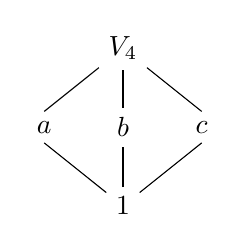
\begin{tikzpicture}[baseline=-0.5ex]
            \node (v4) at (0, 1) {$V_4$};
            \node (a) at (-1, 0) {$\gen a$};
            \node (b) at (0, 0) {$\gen b$};
            \node (c) at (1, 0) {$\gen c$};
            \node (1) at (0, -1) {1};

            \draw (1) -- (a.south);
            \draw (a.north) -- (v4);
            \draw (1) -- (b.south);
            \draw (b.north) -- (v4);
            \draw (1) -- (c.south);
            \draw (c.north) -- (v4);
        \end{tikzpicture}
        \]
        Note that $V_4$ is abelian that is not isomorphic to $Z_4$ since it does not contain elements of order 4.
        \item $S_3$ is the lattice:
        \begin{center}
            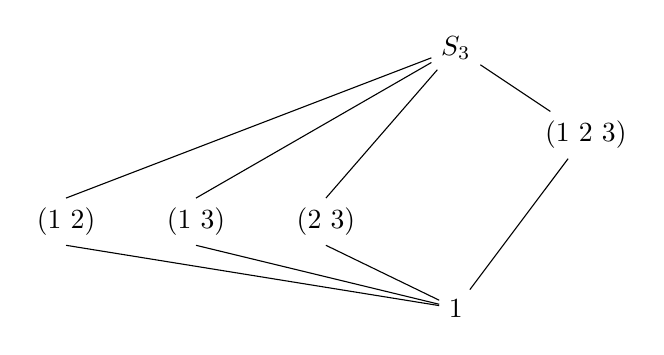
\begin{tikzpicture}[scale = 1.1]
                \node (s3) at (0, 0) {$S_3$};
                \node (12) at (-4.5, -2) {$\gen{(1\ 2)}$};
                \node (13) at (-3, -2) {$\gen{(1\ 3)}$};
                \node (23) at (-1.5, -2) {$\gen{(2\ 3)}$};
                \node (123) at (1.5, -1) {$\gen{(1\ 2\ 3)}$};
                \node (1) at (0, -3) {1};

                \draw (1) -- (12.south);
                \draw (12.north) -- (s3);
                \draw (1) -- (13.south);
                \draw (13.north) -- (s3);
                \draw (1) -- (23.south);
                \draw (23.north) -- (s3);
                \draw (1) -- (123) -- (s3);
            \end{tikzpicture}
        \end{center}
        \item $D_8$ is the lattice:
        \begin{center}
            \begin{tikzpicture}[scale=1.6]
                \node (d8) at (0, 0) {$D_8$};
                \node (sr2) at (-1, -1) {$\gen{s, r^2}$};
                \node (r) at (0, -1) {$\gen r$};
                \node (rsr2) at (1, -1) {$\gen{rs, r^2}$};
                \node (s) at (-2, -2) {$\gen s$};
                \node (r2s) at (-1, -2) {$\gen{r^2s}$};
                \node (r2) at (0, -2) {$\gen{r^2}$};
                \node (rs) at (1, -2) {$\gen{rs}$};
                \node (r3s) at (2, -2) {$\gen{r^3s}$};
                \node (1) at (0, -3) {1};

                \draw (1) -- (s) -- (sr2) -- (d8);
                \draw (1) -- (r2s) -- (sr2);
                \draw (1) -- (r2) -- (sr2);
                \draw (1) -- (rs) -- (rsr2) -- (d8);
                \draw (1) -- (r3s) -- (rsr2);
                \draw (r2) -- (r) -- (d8);
                \draw (r2) -- (sr2);
                \draw (r2) -- (rsr2);
            \end{tikzpicture}
        \end{center}
        \item $Q_8$ is the lattice:
        \begin{center}
            \begin{tikzpicture}[scale=1.25]
                \node (q8) at (0, 0) {$Q_8$};
                \node (i) at (-1, -1) {$\gen i$};
                \node (j) at (0, -1) {$\gen j$};
                \node (k) at (1, -1) {$\gen k$};
                \node (-1) at (0, -2) {$\gen{-1}$};
                \node (1) at (0, -3) {1};

                \draw (1) -- (-1) -- (i.south);
                \draw (i.north) -- (q8);
                \draw (1) -- (-1) -- (j) -- (q8);
                \draw (1) -- (-1) -- (k.south);
                \draw (k.north) -- (q8);
            \end{tikzpicture}
        \end{center}
        \item $D_{16}$ has a lattice that is not a planar graph, or is a graph drawn on a plane without lines crossing. A way of drawing it is
        \begin{center}
            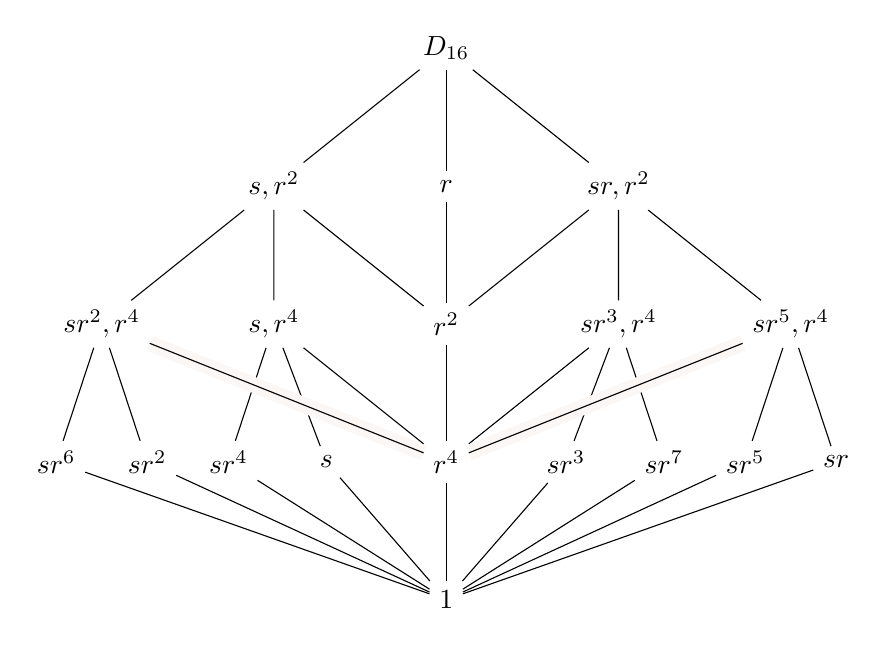
\begin{tikzpicture}[scale=1.75]
                \node (d16) at (0, 0) {$D_{16}$};

                \node (s r2) at (-1.25, -1) {$\gen{s, r^2}$};
                \node (r) at (0, -1) {$\gen r$};
                \node (srr2) at (1.25, -1) {$\gen{sr, r^2}$};

                \node (sr2r4) at (-2.5, -2) {$\gen{sr^2, r^4}$};
                \node (s r4) at (-1.25, -2) {$\gen{s, r^4}$};
                \node (r2) at (0, -2) {$\gen{r^2}$};
                \node (sr3r4) at (1.25, -2) {$\gen{sr^3, r^4}$};
                \node (sr5r4) at (2.5, -2) {$\gen{sr^5, r^4}$};

                \node (sr6) at (-2.83, -3) {$\gen{sr^6}$};
                \node (sr2) at (-2.17, -3) {$\gen{sr^2}$};
                \node (sr4) at (-1.58, -3) {$\gen{sr^4}$};
                \node (s) at (-0.87, -3) {$\gen s$};
                \node (r4) at (0, -3) {$\gen{r^4}$};
                \node (sr3) at (0.87, -3) {$\gen{sr^3}$};
                \node (sr7) at (1.58, -3) {$\gen{sr^7}$};
                \node (sr5) at (2.17, -3) {$\gen{sr^5}$};
                \node (sr) at (2.83, -3) {$\gen{sr}$};

                \node (1) at (0, -4) {1};

                \draw (1) -- (sr6) -- (sr2r4) -- (s r2) -- (d16);
                \draw (1) -- (sr2) -- (sr2r4);
                \draw (1) -- (sr4) -- (s r4) -- (s r2);
                \draw (1) -- (s) -- (s r4);
                \draw (1) -- (r4) -- (r2) -- (r) -- (d16);
                \draw (1) -- (sr3) -- (sr3r4) -- (srr2) -- (d16);
                \draw (1) -- (sr7) -- (sr3r4);
                \draw (1) -- (sr5) -- (sr5r4) -- (srr2);
                \draw (1) -- (sr) -- (sr5r4);
                \draw [preaction={draw, line width=2mm, Tan!10}] (r4) -- (sr2r4);
                \draw (r4) -- (s r4);
                \draw (r4) -- (sr3r4);
                \draw [preaction={draw, line width=2mm, Tan!10}] (r4) -- (sr5r4);
                \draw (r2) -- (s r2);
                \draw (r2) -- (srr2);
            \end{tikzpicture}
        \end{center}
    \end{enumerate}
\end{ex}